% begin module polar-area-ex2
\begin{frame}
\begin{example} %[Example 2, p. 687]
Find the area that lies within the circle $r = 3\sin\theta$ and outside of the cardioid $r = 1+\sin \theta$.
\begin{columns}[c]
\hspace{-.1in}
\column{.3\textwidth}
\psset{xunit=0.9cm, yunit=0.9cm, algebraic=true}
\begin{pspicture}(-2.3, -0.6)(2.3,3.4)
\tiny
\psframe*[linecolor=white](-2.3,-0.6)(2.3,3.4)
\pscustom*[linecolor=\fcColorAreaUnderGraph]{
\parametricplot[linecolor=\fcColorGraph]{2.617993878}{0.523598776}{(1+sin(t))*cos(t)|(1+sin(t))*sin(t)}
\parametricplot[linecolor=\fcColorGraph]{0.523598776}{2.617993878}{(3*sin(t))*cos(t)|(3*sin(t))*sin(t)}
}
\parametricplot[linecolor=\fcColorGraph, plotpoints=1000] {0}{6.283185307}{(1+sin(t))*cos(t)|(1+sin(t))*sin(t)}
\parametricplot[linecolor=\fcColorGraph, plotpoints=1000] {0}{6.283185307}{(3*sin(t))*cos(t)|(3*sin(t))*sin(t)}
\fcAxesStandardNoFrame{-2.3}{-0.5}{2.2}{3.3}
\uncover<2->{
\psline[linecolor=\fcColorTangent](0, 0)(! 2 2 3 sqrt div)
\psline[linecolor=\fcColorTangent](0, 0)(! -2 2 3 sqrt div)
\fcFullDot{1.299038106}{0.75}
\fcFullDot{-1.299038106}{0.75}
\rput[t](1.8, 0.8){$\theta=\frac{\pi}{6}$}
\rput[t](-1.8, 0.8){$\theta=\frac{5\pi}{6}$}
}
\rput[l](1, 2.8){$r=3\sin\theta$}
\rput[t](-1.2, -0.35){$r=1+\sin\theta$}
\end{pspicture}
%\ \uncover<2->{%
%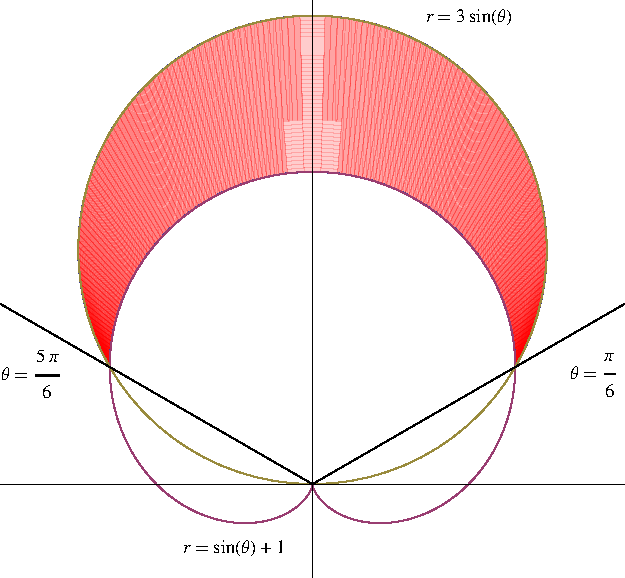
\includegraphics[height=4cm]{polar-curves/pictures/11-04-ex2.pdf}%
%}%

\uncover<2->{%
The curves meet if
\abovedisplayskip=0pt
\belowdisplayskip=0pt
\begin{eqnarray*}
3\sin \theta & = & 1 + \sin \theta\\
\sin \theta & = & \frac{1}{2}\\
\theta & = &\frac{\pi}{6}, \ \frac{5\pi}{6}
\end{eqnarray*}
}%
\column{.65\textwidth}
%\begin{eqnarray*}
$
{\renewcommand{\arraystretch}{1.7}
\begin{array}{l}
 \uncover<3->{ A = } %
\uncover<3->{%
\frac{1}{2}\int_{\frac{\pi}{6}}^{\frac{5\pi}{6}}(3\sin \theta )^2\diff \theta%
%}\\%
%&&\uncover<3->{%
- \frac{1}{2}\int_{\frac{\pi}{6}}^{\frac{5\pi}{6}}(1+\sin \theta )^2\diff \theta%
}\\%
 \uncover<4->{\phantom{A} = } %
\uncover<4->{%
\frac{1}{2} \int_{\frac{\pi}{6}}^{\frac{5\pi}{6}}\left( 9\sin^2\theta - (1 + 2\sin \theta + \sin^2\theta)\right)\diff \theta%
}\\%
 \uncover<5->{\phantom{A} = } %
\uncover<5->{%
\alert<handout:0| 6>{\frac{1}{2}} \int_{\alert<handout:0| 6>{\frac{\pi}{6}}}^{\alert<handout:0| 6>{\frac{5\pi}{6}}}\left( 8\sin^2\theta - 1 - 2\sin \theta\right)\diff \theta%
}\\%
 \uncover<6->{\phantom{A} = } %
\uncover<6->{%
\int_{\alert<handout:0| 6>{\frac{\pi}{6}}}^{\alert<handout:0| 6>{\frac{\pi}{2}}}\left( \alert<handout:0| 7>{8\sin^2\theta - 1} - 2\sin \theta\right)\diff \theta%
}\\%
 \uncover<7->{\phantom{A} = } %
\uncover<7->{%
\int_{\alert<handout:0| 6>{\frac{\pi}{6}}}^{\alert<handout:0| 6>{\frac{\pi}{2}}}\left( \alert<handout:0| 7>{3 - 4\cos 2\theta } - 2\sin \theta\right)\diff \theta%
}\\%
 \uncover<8->{\phantom{A} = } %
\uncover<8->{%
\left[ 3\alert<handout:0| 9-10,15-16>{\theta} - 2\alert<handout:0| 11-12,17-18>{\sin 2\theta} + 2\alert<handout:0| 13-14,19-20>{\cos \theta} \right]_{\alert<handout:0| 15-20>{\frac{\pi}{6}}}^{\alert<handout:0| 9-14>{\frac{\pi}{2}}}%
}\\%
 \uncover<9->{\phantom{A} = } %
\uncover<9->{%
\left( 3\alert<handout:0| 10>{\uncover<10->{\frac{\pi}{2}}} - 2\cdot \alert<handout:0| 12>{\uncover<12->{0}} + 2\cdot \alert<handout:0| 14>{\uncover<14->{0}}\right) - \left( 3\alert<handout:0| 16>{\uncover<16->{\frac{\pi}{6}}} - 2\alert<handout:0| 18>{\uncover<18->{\frac{\sqrt{3}}{2}}} + 2\alert<handout:0| 20>{\uncover<20->{\frac{\sqrt{3}}{2}}}\right)%
}\\%
 \uncover<21->{\phantom{A} = } %
\uncover<21->{%
\pi%
}%
\end{array}
}%
$
\end{columns}
\end{example}
\end{frame}
% end module polar-area-ex2
